\section{Evaluation}
\label{sec:results}
\subsection{Experimental Setup}
\begin{table}[]
    \begin{tabular}{@{}ccccc@{}}
        \toprule
        WBS   & TCAS      & replace      & NanoXML   &            \\ \midrule
        1234  & 4509      & 3980         & 871       &            \\ \midrule
        Siena & Schedule2 & PrintTokens2 & ApacheCLI & MerArbiter \\ \midrule
        1551  & 722       & 1180         & 910       & 20639      \\ \bottomrule
    \end{tabular}
    \caption{Static analysis time (msec) for all 9 benchmarks}
    \label{table:static-analysis-time}
\end{table}
%
We implemented the above mentioned transformations as a wrapper around the Symbolic PathFinder~\cite{spf} tool.
%
To make use of region summaries in Symbolic PathFinder, we use an existing feature of SPF named \textit{listener}.
%
A listener is a method defined within SPF that is called for every bytecode instruction executed by SPF.
%
Java Ranger adds a path merging listener to SPF that, on every instruction, checks (1) if the instruction involves
checking a symbolic condition, and (2) if Java Ranger has a pre-computed static summary that begins at that
instruction\rq s bytecode offset.
%
If both of these conditions are satisfied, Java Ranger instantiates the multi-path region summary corresponding to that
bytecode offset by reading inputs from and writing outputs to the stack and the heap.
%
It then conjuncts the instantiated region summary with the path condition and resumes symbolic execution at the
bytecode offset of the end of the region.
%
Our implementation, named \tool, wraps around SPF and can be configured to run in the following five modes.\\
%
\textbf{Mode 1}: \tool\ runs vanilla SPF without any path merging.\\
%
\textbf{Mode 2}: \tool\ summarizes multi-path regions with a single exit point and instantiates them if they are encountered.
This includes multi-path regions that have local, stack, field, or array outputs.
%
\tool\ substitutes local inputs into the Ranger IR representation of the multi-path region, and constructs SSA form
Ranger IR for all field and array accesses in the region using its instantiation-time context.
%
The SSA form representation of all field and array accesses allows the Ranger IR to be simplified uniformly across all
variable types which reduces the size of the region summary and improves the performance of \tool.
%
While our current implementation of \tool\ cannot instantiate summaries with symbolic object and array
references, it is capable of summarizing reads and writes to arrays with symbolic indices.\\
%
\textbf{Mode 3}: In addition to using summaries instantiated in mode 2, \tool\ instantiates all multi-path region
summaries that make method calls which have also been statically summarized.
%
Method summaries, that have a single exit point in the form of a control-flow returning instruction, are inlined into
the multi-path region summary based on the instantiation-time type of the method.\\
%
\textbf{Mode 4}: In addition to using summaries instantiated in mode 3, \tool\ uses single-path cases to allow
regions to have more than one exit point.
%
These exit points take the form of new object allocations and exceptional behavior present in the region.\\
%
\textbf{Mode 5}: In addition to using summaries instantiated in mode 4, \tool\ converts multiple exit points that return
control flow into a single control flow-returning exit point to allow multi-path regions to have more than one non-returning exit point.

We used the control-flow graph recovered by Wala~\cite{Wala} to bootstrap our static statement recovery process.
%
While our static statement recovery was able to summarize thousands of regions in Java library code, many of these
summaries could not be instantiated due to JPF\rq s use of native peers~\cite{jpf-mji}.
%
To avoid these unnecessary instantiation failures and target our static statement recovery towards the benchmark code,
we turned off statement recovery across a few Java library packages in Wala on all benchmarks.

We ran the above implementation using the incremental solving mode of Z3 using the bitvector theory.
%
The incremental solving mode provides only the last constructed constraint to the solver instead of passing the entire
path condition every time a query is to be solved.
%
Since path-merging can create large formulas in the path condition, the incremental solving mode was beneficial in
reducing the number of times large formulas had to be passed to the solver.
%
\subsection{Evaluation}
%
In order to evaluate the performance of \tool, we used the following nine benchmarking programs commonly used to
evaluate symbolic execution performance.
%
Eight of these programs were provided by Wang et al.~\cite{dgse} which also includes a translation of the
Siemens suite to Java.
%
(1) Wheel Brake System (WBS)~\cite{yang2014directed} is a synchronous reactive
component developed to make aircraft brake safely when taxing, landing, and during a rejected take-off.
%
(2) Traffic Collision Avoidance System (TCAS) is part of a suite of programs commonly referred to as the Siemens
suite~\cite{siemens-benchmarks}. TCAS is a system that maintains altitude separation between aircraft to avoid mid-air
collisions.
%
(3) Replace is another program that\rq s part of the Siemens suite. Replace searches for a pattern in a given input and
replaces it with another input string.
%
(4) NanoXML is an XML Parser written in Java which consists of 129 procedures and 4608 lines of code.
%
(5) Siena~(Scalable Internet Event Notification Architecture) is an Internet-scale event notification middleware for
distributed event-based applications~\cite{siena} which consists of 94 procedures and 1256 lines of code.
%
(6) Schedule2 is a priority scheduler which consists of 27 procedures and 306 lines of code.
%
(7) PrintTokens2 is a lexical analyzer which consists of 30 procedures and 570 lines of code.
%
(8) ApacheCLI~\cite{apachecli} provides an API for parsing command lines options passed to programs.
It consists of 183 procedures and 3612 lines of code.
%
(9) MerArbiter models a flight software component of NASA JPL\rq s Mars Exploration Rovers.
%
%It was originally modeled in Simulink/Stateflow and automatically translated into Java using the Polyglot framework.
%
We used the version made
available by Yang et al.~\cite{memoise}. This benchmark consists of 268 classes, 553 methods, 4697 lines of code
including the Polyglot framework.

We first ran each of these benchmarks using SPF with increasing number of symbolic inputs and obtained the most number of inputs
with which SPF finished complete exploration of each benchmark within a 12 hour time budget.
%
We then ran each benchmark with this number of symbolic inputs with \tool.
%
This evaluation allowed us to check if \tool\ is faster than SPF at achieving complete path exploration of each benchmark.
%
Next, we used the fastest mode of \tool\ to check if it could explore the benchmark with even more symbolic inputs within
the same 12 hour time budget.
%
We report results from both of these evaluations for each benchmark in Figures~\ref{fig:results1},~\ref{fig:results2}.
%
Detailed experimental results are reported in Tables~\ref{table:results1},~\ref{table:results2} in a file named
``results-tables.pdf'' in the supplementary material included in our submission.
%
A even more detailed set of results can be found in a file named ``results-all.csv''.
%
Since Java Ranger relies on a prior static analysis to construct region summaries, we report the time taken to statically
analyze all the code in each of the benchmarks in Table~\ref{table:static-analysis-time}.
%
We found that the total time required for static analyis is roughly proportional to the size of the benchmark.
%
While such static analysis performance can cause \tool\ to be slower on benchmarks with a small number of execution
paths, we found that the cost of static analysis gets amortized as the number of execution paths increased.
%
\begin{figure*}%
    \centering
    \subfloat[\tool\ explores WBS with one execution path in modes 2, 3, 4, and 5 regardless of the number of
    symbolic inputs. \tool\ doesn't need to query the solver in modes 2, 3. WBS-s15-m1 times out in 12 hours.]{
        {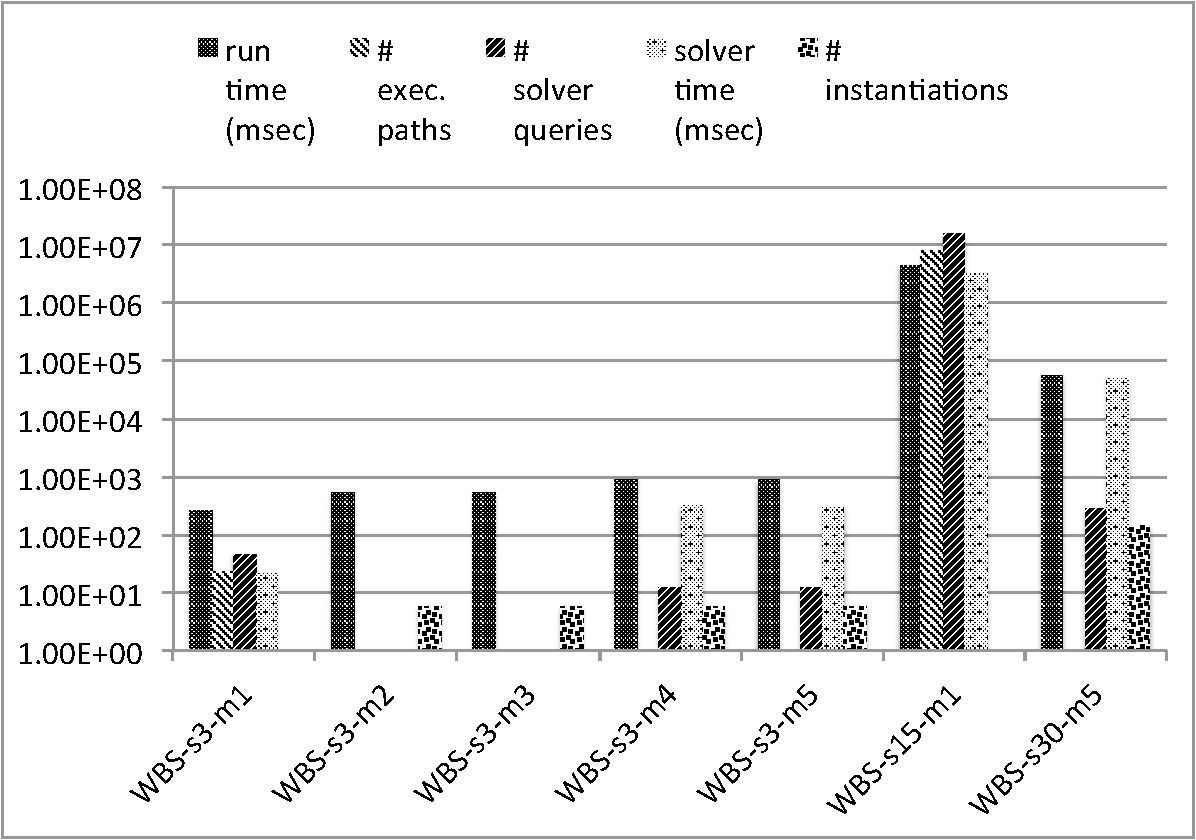
\includegraphics[width=\columnwidth]{figures/wbs-results.pdf}
        \label{fig:wbs-results}}}%
    \hfill
    \subfloat[\tool\ summarizes TCAS in one execution path starting with mode 3
    regardless of the number of symbolic inputs. TCAS-s24-m1 times out in 12 hours. In mode 3, \tool\ uses 28 method summaries
    in every step of TCAS.]{
        {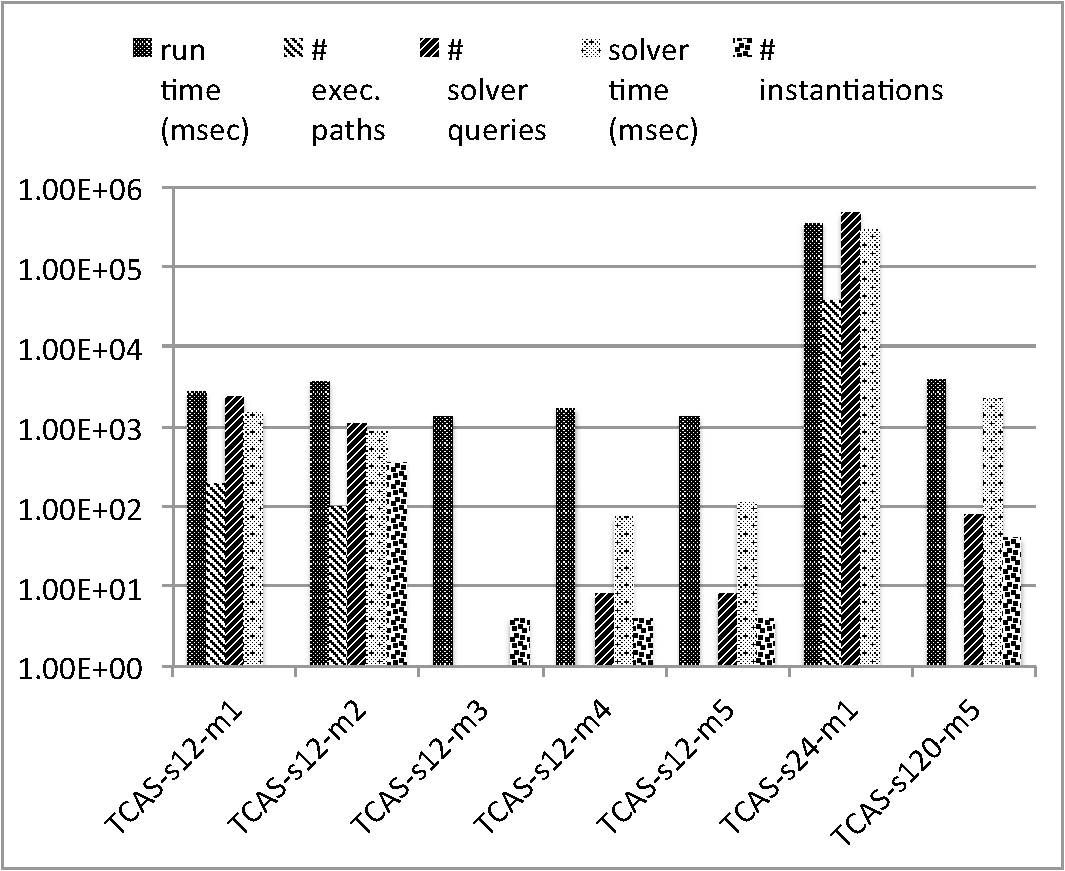
\includegraphics[width=\columnwidth]{figures/tcas-results.pdf} }
        \label{fig:tcas-results}}%
    \hfill
    \subfloat[In mode 2, \tool\ reduces the execution path count in Replace by 37\% from mode 1 with a modest decrease
    in running time of 13\%. In modes 4, 5, \tool\ reduces the execution path count by an overall 89\% at the expense of more
    a larger path condition caused due to more region instantiations.]{
        {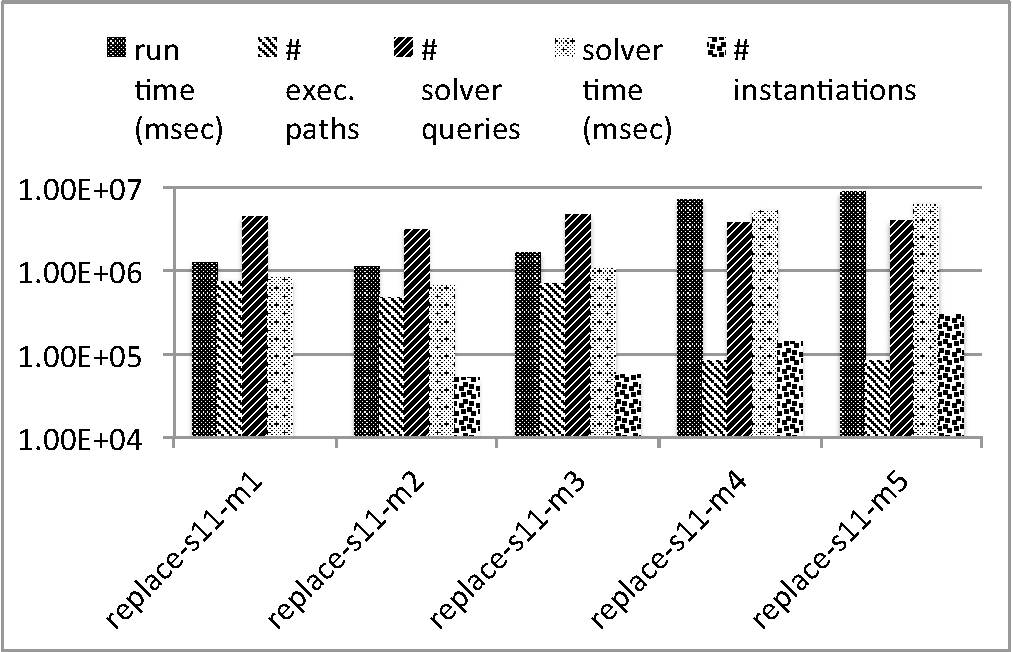
\includegraphics[width=\columnwidth]{figures/replace-results.pdf} }
        \label{fig:replace-results}}%
    \hfill
    \subfloat[In mode 5, \tool\ reduces the execution path count in NanoXML with 7 symbolic inputs by 85\% while
    reducing running time by 40\%. This improvement is due to conversion of multiple control-flow returning exit points
    in multi-path regions into a single control-flow returning exit point in mode 5.]{
    {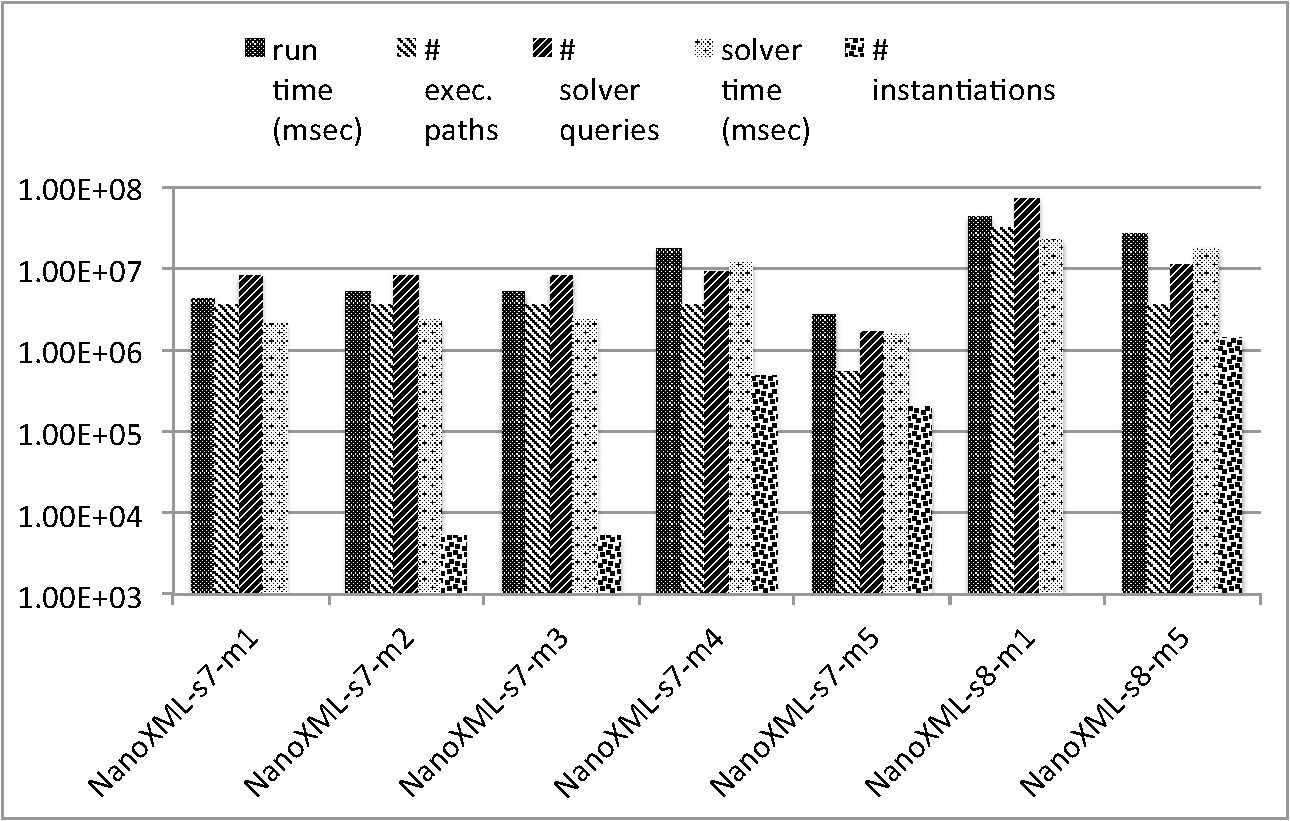
\includegraphics[width=\columnwidth]{figures/nanoxml-results.pdf}
    \label{fig:nanoxml-results}}}%
    \hfill
    \subfloat[\tool\ introduces a 3\% overhead in running time with Siena. The overhead is more with Schedule2 because
    of its short runtime in mode 1 and because \tool\ needs about the same amount of time for its offline static analysis
    in mode 5.]{
    {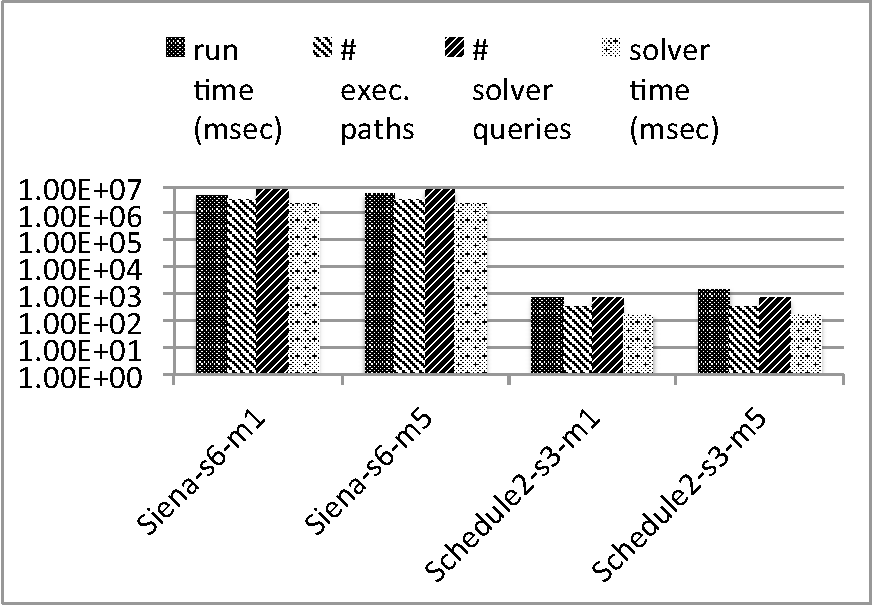
\includegraphics[width=\columnwidth]{figures/siena-schedule2-results.pdf} }
    \label{fig:siena-schedule2-results}}%
    \hfill
    \subfloat[While \tool\ reduces the execution path count by 10\% in modes 2, 3, 4, and by 27\% in mode 5, this
    reduction comes at the expense of longer formulas sent to the solver without achieving a significant reduction in
    the number of solver queries.]{
    {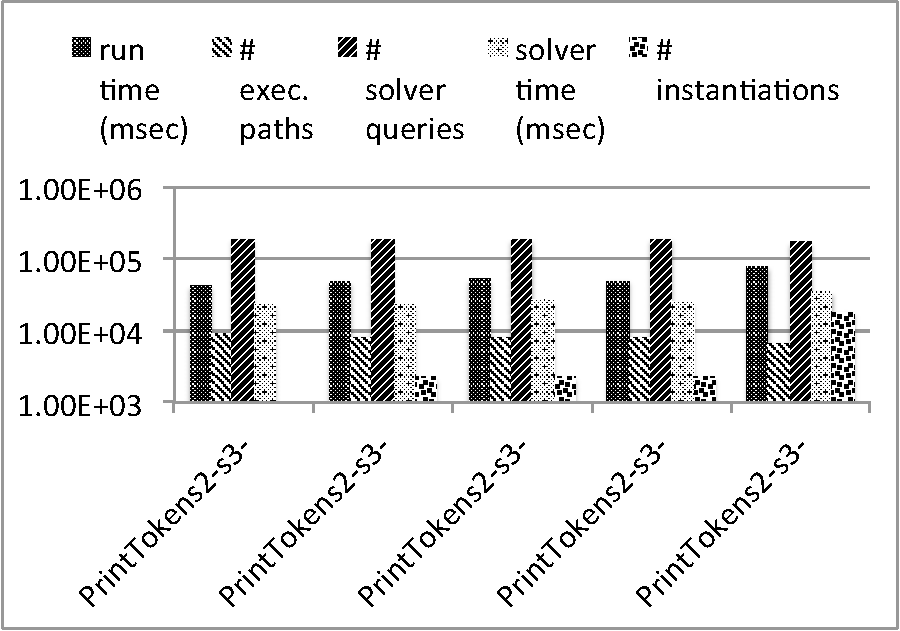
\includegraphics[width=\columnwidth]{figures/printtokens2-results.pdf} }
    \label{fig:printtokens2-results}}%
    \caption{Performance of \tool\ on WBS, TCAS, Replace, NanoXML, Siena, Schedule, PrintTokens2 as shown by using a
    <benchmark-name>-s<number of symbolic inputs>-m<\tool\ mode> format. \tool\ runs vanilla SPF in mode 1.}%
    \label{fig:results1}%
\end{figure*}
%
\begin{figure}[]%
    \centering
    \subfloat[In mode 2 in ApacheCLI with 6 symbolic inputs, \tool\ reduces execution path count by 96\% while reducing
    running time by 86\%. While vanilla SPF (mode 1 in \tool) times out in 12 hours with 7 symbolic inputs, \tool\
    manages to finish in 3.6 hours in mode 2.]{
    {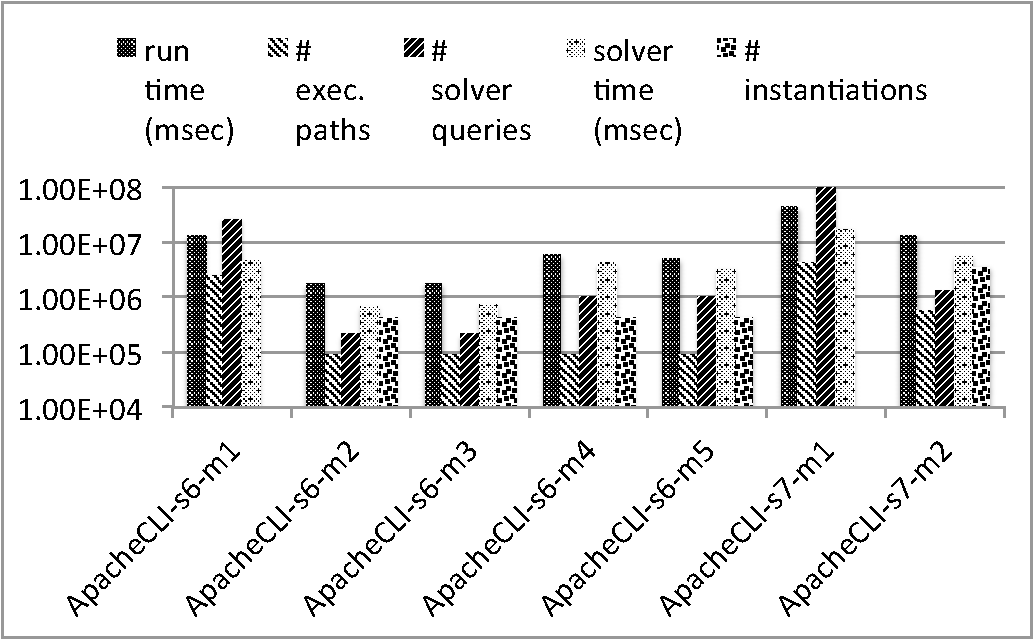
\includegraphics[width=\columnwidth]{figures/apachecli-results.pdf}
    \label{fig:apachecli-results}}}%
    \qquad
    \subfloat[The last input to ApacheCLI is different from all the other inputs because it controls whether ApacheCLI
    should stop on encountering a non-option input. The benefits of using \tool\ with ApacheCLI are still evident
    if this input is made symbolic. In mode 2, \tool\ reduces execution path count by 96\% and running time by 88\%.
    Vanilla SPF (mode 1 in \tool) still times out in 12 hours with 8 symbolic inputs (including the {\tt stopOnNonOption}
    input while \tool\ manages to finish in 7.2 hours in mode 2.)]{
    {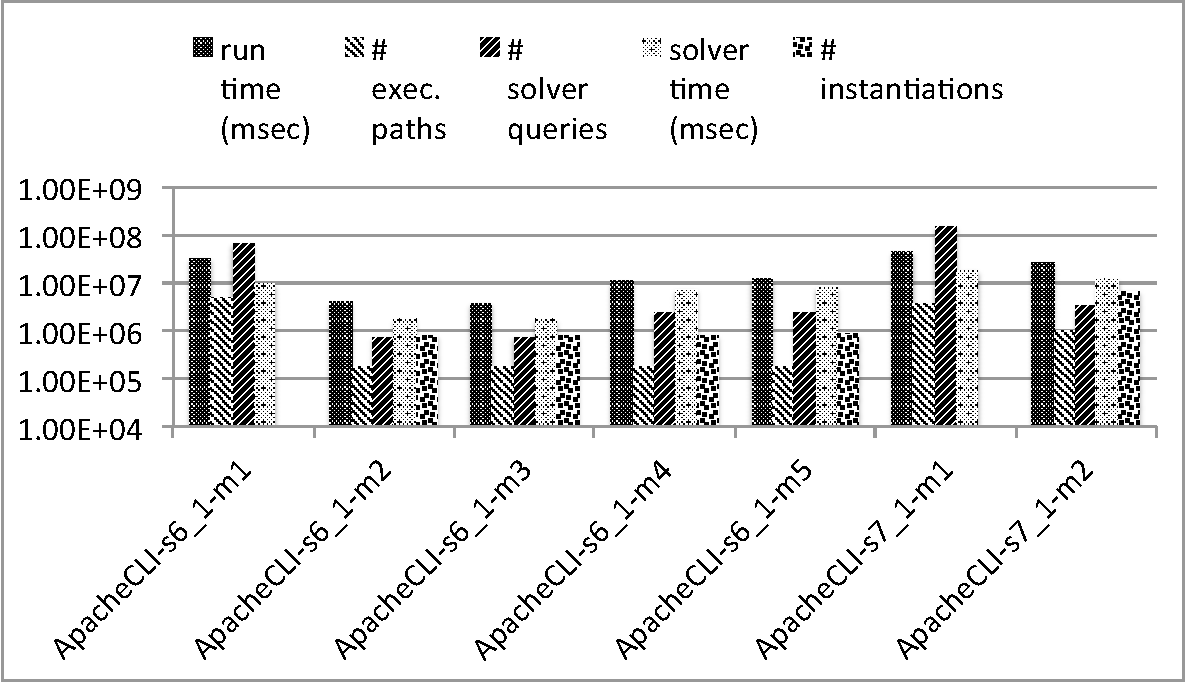
\includegraphics[width=\columnwidth]{figures/apachecli-1-results.pdf} }
    \label{fig:apachecli-1-results}}%
%    \qquad
    \caption{Performance of \tool\ on ApacheCLI}%
    \label{fig:results2}%
\end{figure}
\begin{figure}
%    \subfloat[With 6 steps (24 symbolic inputs) of MerArbiter, \tool\ reduces execution path count by 94\% and running time by 68\%. While
%    vanilla SPF (mode 1 in \tool) times out in 12 hours with 7 steps (28 symbolic inputs), \tool finishes in 3.4\% hours
%    in mode 2.]{
    {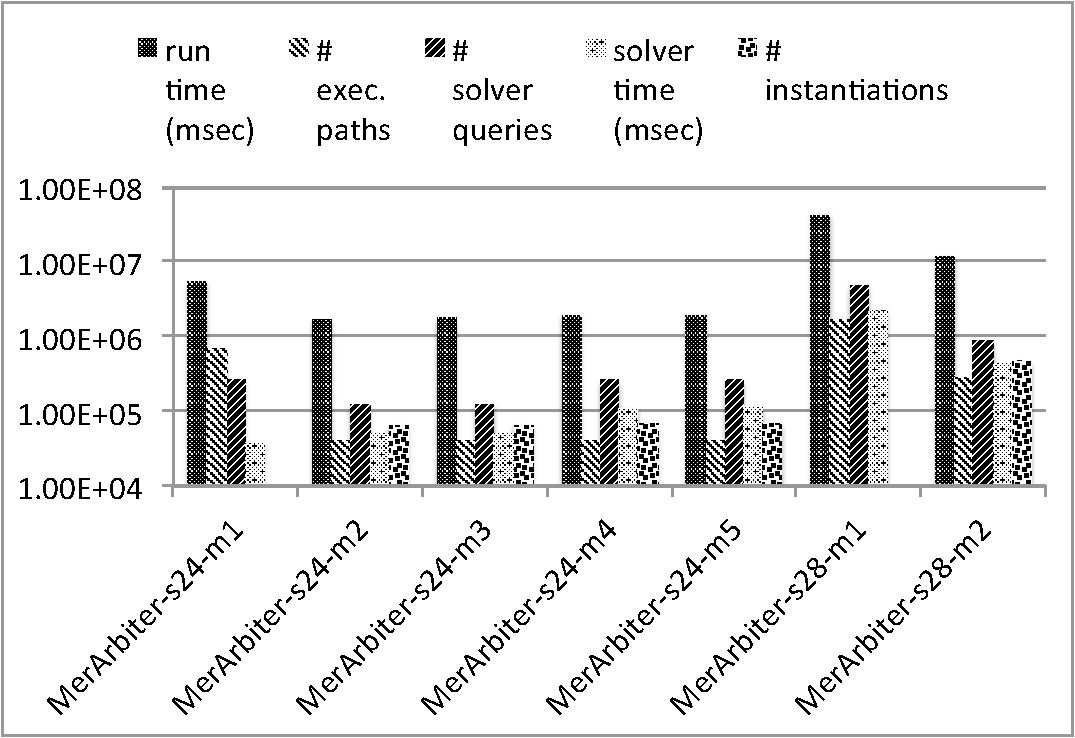
\includegraphics[width=\columnwidth]{figures/merarbiter-results.pdf} }
    \label{fig:merarbiter-results}%
    \caption{With 6 steps (24 symbolic inputs) of MerArbiter, \tool\ reduces execution path count by 94\% and running time by 68\%.
    SPF times out in 12 hours with 7 steps (28 inputs), \tool\ finishes in 3.4 hours in mode 2.}
\end{figure}

Figures~\ref{fig:results1},~\ref{fig:results2} show that \tool\ achieves a significant speed-up over SPF with
5~(WBS, TCAS, NanoXML, ApacheCLI, MerArbiter) of the 9 benchmarks in terms of both running time and number of
execution paths.
%
Of the remaining four benchmarks, in the replace benchmark, \tool\ achieves a modest reduction in execution time
of 13\% while reducing the number of execution paths by 37\% in mode 2.
%
In mode 5, while it reduces the number of execution paths by about 89\%, it incurs an increase in execution time due to
an increase in formula size caused due to an increase in the number of region instantiations in mode 5.
%
On manually investigating the set of instantiated regions in replace, we found that the outputs of most regions were
being branched on later in the code causing the benefit from more instantiations to be lost.
%
Similar reasons cause \tool\ to lose out on a reduction in running time while reducing the execution path
count with the PrintTokens2 benchmark.

\tool\ has the same performance as SPF on Siena and Schedule2 with a 3\% overhead in running time that comes from
\tool\rq s lookup of a region summary for every executed branch instruction and recording of instantiation-time metrics.
%
We restrict our results with Siena to 6 symbolic inputs because 6 is the most number of symbolic inputs for which
SPF finishes complete path exploration within a 12 hour time budget.
%
On running Siena, the overhead of \tool\ results from running into (1) 3,800,343 symbolic branch
instructions that a region summary lookup and (2) 8,959,692 concrete branch instructions that
\tool\ could have summarized, had these branches been symbolic.

\tool\ is able to summarize the entire step function of WBS and TCAS into a single execution path.
%
In case of WBS, \tool\ summarizes a multi-path region that consists of 9 branches.
%
In case of TCAS, \tool\ uses 28 method summaries in each step of TCAS, many of which summarize multiple return values
into a single formula that represents all the feasible return values of the method.
%
While SPF does not finish more than 5 steps of WBS and 2 steps of TCAS within 12 hours, \tool\ finishes 10 steps of both
benchmarks within 59 seconds and 5.6 seconds respectively.

On the NanoXML benchmark, \tool\ finds several opportunities for execution path count reduction on account of the
NanoXML benchmark having several methods with multi-path regions that have a control-flow returning instruction on every
branch side.
%
With mode 5 of \tool\ converting such multiple control-flow returning exit points regions into a single control-flow
returning exit point, \tool\ is able to use more than 27,000 method summaries when running NanoXML with 8 symbolic
inputs and achieve complete path exploration in 7.3 hours while vanilla SPF~(which is the same as mode 1 of \tool)
times out.

On the ApacheCLI benchmark, the most significant benefit is introduced in mode 2 of \tool.
%
Modes 4, 5 cause an increase in execution path count and running time but still give a significant reduction over
mode 1.
%
The increase in running time in modes 4 and 5 results from \tool\rq s use of the solver to check if the single-path cases
in modes 4 and 5 are feasible.
%
In the future, we plan to use a counter-example cache to reduce the use of a solver to check the feasibility of these
single-path cases.

In the MerArbiter benchmark, while the most significant benefit is introduced in mode 2 of \tool, the benefit in terms of
both execution path count and running time remains the same in modes 3, 4, and 5.
%
All the multi-path regions that SPF~(or mode 1 in \tool) needs to branch on but are summarized by \tool\ are small
regions that compute a boolean value based on a symbolic branch and write it to the stack as an operand to be used
by the following return instruction.
%
Most of these multi-path regions lie inside several levels of nested classes and field references that necessitate
a fixed-point computation over the field substitution and constant propagation transformations.
%
\tool\ summarizes such multi-path regions and does 464,000 instantiations with 7 steps of MerArbiter, with more than
319,000 instantiations needing more than 8 iterations of the fixed-point computation.